\documentclass[11pt]{article}

\usepackage[a4paper,margin=1in]{geometry}
\usepackage[T1]{fontenc}
\usepackage{lmodern}
\usepackage{microtype}
\usepackage{booktabs}
\usepackage{tabularx}
\usepackage{longtable}
\usepackage{enumitem}
\usepackage{xcolor}
\usepackage{parskip}
\usepackage{pdflscape}
\usepackage{tikz}
\usetikzlibrary{positioning,arrows.meta,fit,backgrounds,calc}
\usepackage[hidelinks]{hyperref}

\definecolor{accent}{RGB}{30,80,140}
\definecolor{okgreen}{RGB}{30,120,60}
\definecolor{warn}{RGB}{170,90,10}
\definecolor{gap}{RGB}{160,40,40}
\definecolor{harnesscol}{RGB}{110,70,160}
\hypersetup{colorlinks=true,urlcolor=accent,linkcolor=accent}

\newcommand{\code}[1]{\texttt{#1}}
\newcommand{\done}{\textcolor{okgreen}{\textbf{done}}}
\newcommand{\partialx}{\textcolor{warn}{\textbf{partial}}}
\newcommand{\gapx}{\textcolor{gap}{\textbf{gap}}}
\newcommand{\EX}{\textcolor{okgreen}{\textbf{existing}}}
\newcommand{\BU}{\textcolor{accent}{\textbf{built}}}
\newcommand{\PL}{\textcolor{warn}{\textbf{planned}}}
\newcommand{\arw}{$\rightarrow$}
\newcommand{\dt}{$\cdot$}
\setlist[itemize]{leftmargin=1.35em,itemsep=2pt,topsep=3pt}

\tikzset{
  wbox/.style={rectangle, rounded corners=2pt, draw, align=center,
               text width=25mm, minimum height=10mm, inner sep=3pt, line width=0.5pt},
  existing/.style={wbox, fill=okgreen!12, draw=okgreen!75!black},
  built/.style={wbox, fill=accent!12, draw=accent!75!black},
  planned/.style={wbox, fill=warn!16, draw=warn!75!black, dash pattern=on 2.2pt off 1.6pt},
  io/.style={wbox, fill=black!7, draw=black!45, text width=17mm},
  layer/.style={rectangle, rounded corners=3pt, draw, align=left, inner sep=6pt,
                text width=122mm, line width=0.6pt},
  harness/.style={layer, fill=harnesscol!10, draw=harnesscol!75!black,
                  dash pattern=on 3pt off 2pt},
  toollayer/.style={layer, fill=accent!10, draw=accent!75!black},
  extsw/.style={layer, fill=black!6, draw=black!45},
  ar/.style={-{Stealth[length=2.2mm]}, line width=0.7pt, draw=black!55},
}

\title{\vspace{-1.2cm}\textbf{\LARGE Agentic Lagrangian Extraction from the Literature}\\[4pt]
\large Midterm Progress Report \& Technical Design}
\author{}
\date{}

\begin{document}
\maketitle
\vspace{-2.1cm}

\begin{center}
\begin{tabularx}{\textwidth}{@{}lX@{}}
\textbf{Program} & Google Summer of Code 2026 \quad|\quad ML4SCI \quad|\quad HEPSIM5 \\
\textbf{Contributor} & Ken Wu \\
\textbf{Mentors} & S.~Mrenna (Fermilab), K.~Matchev, A.~Roman, T.~Menzo (Alabama/Fermilab), I.~Pang (Rutgers) \\
\textbf{Framework} & HEPTAPOD (\code{github.com/tonymenzo/heptapod}) \quad|\quad 350 hours, Advanced \\
\end{tabularx}
\end{center}

\hrulefill

\section{Executive summary}

The project automates a manual high-energy-physics bottleneck: turning a
Beyond-Standard-Model (BSM) scenario into a validated FeynRules \code{.fr}
simulation model. Given a scenario, an agent searches the literature, extracts
the Lagrangian and its conventions, generates a syntactically correct \code{.fr}
file, and validates it.

The central design choice is to be \textbf{harness-agnostic by construction}: we
did not build an orchestrator. We built a layer of deterministic,
schema-validated \emph{tools}, exposed via the Model Context Protocol (MCP), plus
a workflow \emph{prompt}. The ``brain'' that sequences the tools, reads their
errors, and runs the repair loop is a general agent harness---Claude Code,
Codex, Cursor, or the Orchestral runtime---and it is \textbf{pluggable}
(Section~\ref{sec:harness}). This keeps the reasoning where harnesses already
excel and keeps the physics deterministic and reproducible in tools.

\textbf{At midterm, the front half of the pipeline is built and tested} as
HEPTAPOD tools: literature retrieval, schema-constrained extraction, and
deterministic \code{.fr} generation, plus the workflow prompt and a benchmark
scaffold (Section~\ref{sec:progress}). The remaining half---physics-level
validation, benchmarking against reference implementations, and extraction
robustness---is scoped for the second half (Section~\ref{sec:remaining}). This
report also folds in an adversarial self-review that reshaped several choices
(Sections~\ref{sec:novelty}--\ref{sec:doability}).

\section{Progress against the project spec}
\label{sec:progress}

Honest status against the six task ideas and four expected results.

\begin{center}
\renewcommand{\arraystretch}{1.25}
\begin{tabularx}{\textwidth}{@{}p{5.2cm}cX@{}}
\toprule
\textbf{Spec item} & \textbf{Status} & \textbf{Notes} \\
\midrule
1. Survey FeynRules models, catalog conventions & \gapx & Design informed by round-tripping one reference model; a catalog \emph{artifact} (parsed from the FeynRules DB) is now the first second-half task. \\
2. Tool modules: literature search, extraction, \code{.fr} generation & \done & \code{ArxivSearchTool}, \code{FetchPaperPDFTool}, \code{ExtractPaperTextTool}; \code{ExtractLagrangianTool}; \code{FeynRulesModel} schema $+$ \code{GenerateFeynRulesModelTool}. INSPIRE reused. Wired into \code{toolkit.yaml}; tests pass. \\
3. Agent workflow: scenario \arw{} validated model & \partialx & Workflow prompt $+$ harness-run repair loop $+$ Orchestral demo exist; one end-to-end live run $+$ committed artifacts still to do. \\
4. Validation: spectrum, gauge invariance, widths/xsec & \partialx & \code{ValidateModelTool} compiles \code{.fr}\arw{}UFO $+$ checks files/particles. Gauge-invariance and width/cross-section reproduction are second-half (Section~\ref{sec:doability}). \\
5. Test vs benchmark models in the FeynRules DB & \partialx & Eval scores extraction vs.\ hand-authored expectations; diffing against the reference \code{.fr}/UFO (SLQrules, 2HDM, DMsimp) is the planned upgrade. \\
6. Audit trail & \partialx & Detailed protocol in the workflow prompt; making it tool-emitted (\code{audit.json}) is a small task. \\
\bottomrule
\end{tabularx}
\end{center}

\section{Architecture: a harness-agnostic tool layer}
\label{sec:arch}

\subsection{The harness boundary --- what is swappable}
\label{sec:harness}

The system separates cleanly into three layers. Everything that is
\emph{reasoning}---deciding the next tool, reading a FeynRules error, running the
repair loop---belongs to a swappable agent harness. Everything that is a
\emph{deterministic capability}---search, \code{.fr} generation, compilation and
validation---stays a fixed tool. External physics software is reused unchanged.

\begin{figure}[h]
\centering
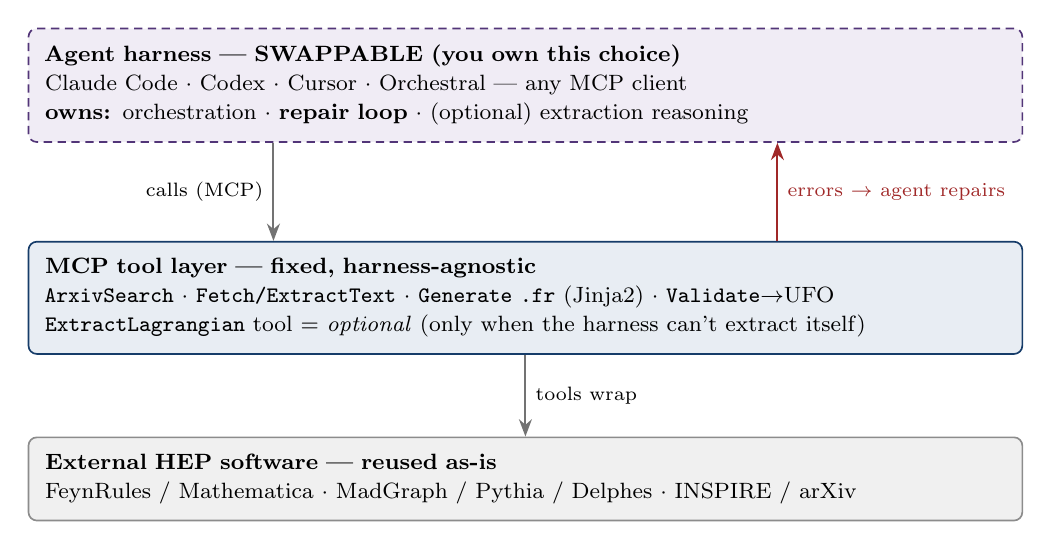
\begin{tikzpicture}[font=\footnotesize]
  \node[harness] (h) at (0,0)
    {\textbf{Agent harness --- SWAPPABLE (you own this choice)}\\[1pt]
     Claude Code \dt{} Codex \dt{} Cursor \dt{} Orchestral --- any MCP client\\[1pt]
     \textbf{owns:} orchestration \dt{} \textbf{repair loop} \dt{} (optional) extraction reasoning};
  \node[toollayer] (t) at (0,-2.7)
    {\textbf{MCP tool layer --- fixed, harness-agnostic}\\[1pt]
     \code{ArxivSearch} \dt{} \code{Fetch/ExtractText} \dt{} \code{Generate .fr} (Jinja2) \dt{} \code{Validate}\arw{}UFO\\[1pt]
     \code{ExtractLagrangian} tool $=$ \emph{optional} (only when the harness can't extract itself)};
  \node[extsw] (e) at (0,-5.0)
    {\textbf{External HEP software --- reused as-is}\\[1pt]
     FeynRules / Mathematica \dt{} MadGraph / Pythia / Delphes \dt{} INSPIRE / arXiv};
  \draw[ar] ([xshift=-32mm]h.south) -- ([xshift=-32mm]t.north)
     node[midway,left,font=\scriptsize]{calls (MCP)};
  \draw[ar, draw=gap] ([xshift=32mm]t.north) -- ([xshift=32mm]h.south)
     node[midway,right,font=\scriptsize,text=gap]{errors \arw{} agent repairs};
  \draw[ar] (t.south) -- (e.north) node[midway,right,font=\scriptsize]{tools wrap};
\end{tikzpicture}
\caption{The swap boundary. The \textcolor{harnesscol}{\textbf{harness}} (dashed,
top) is interchangeable and owns all reasoning, including the repair loop; the
\textcolor{accent}{\textbf{MCP tool layer}} is built once and reused by any
harness; external software is untouched. Because there is no bespoke
orchestrator, swapping Orchestral for Claude Code or Codex is a configuration
change, not a rewrite.}
\end{figure}

\noindent\textbf{The repair loop is the harness's job, and already is.} There is
no hand-written repair control-flow. The loop is specified in the workflow
prompt, and whichever harness runs that prompt executes it: generate \code{.fr}
\arw{} validate \arw{} read the concrete error \arw{} fix the model \arw{}
regenerate. The tools exist to feed that loop actionable, structured errors:
\code{GenerateFeynRulesModelTool} returns Pydantic validation failures,
\code{ValidateModelTool} returns \code{\{passed, checks[], feynrules\_log\}}. This
is exactly the edit\,\arw{}run\,\arw{}read-failure\,\arw{}fix loop coding agents
are built for, so Claude Code / Codex perform it natively.

\noindent\textbf{One tool is deliberately optional: \code{ExtractLagrangianTool}.}
It embeds its own model call (schema-constrained decoding). When a capable
coding-agent harness drives the pipeline, that is redundant---the harness reads
the extracted paper text and emits the \code{FeynRulesModel} JSON itself. We keep
the tool only for the headless/batch path (e.g.\ scoring many papers with a
\emph{pinned} model for reproducible benchmark numbers).

\noindent\textbf{Two operating modes, same tools.} Interactive / demo / midterm
work is driven by \textbf{Claude Code or Codex} (strongest models, native repair
loop, fully visible). Reproducible benchmarking uses the \textbf{Orchestral /
thin owned loop} with a pinned model and logged traces, so eval numbers
reproduce. This is the ``harness-as-dev-tool vs.\ harness-as-reproducible-runtime''
distinction, realized on one MCP tool layer.

\subsection{End-to-end workflow}

\begin{landscape}
\begin{figure}[p]
\centering
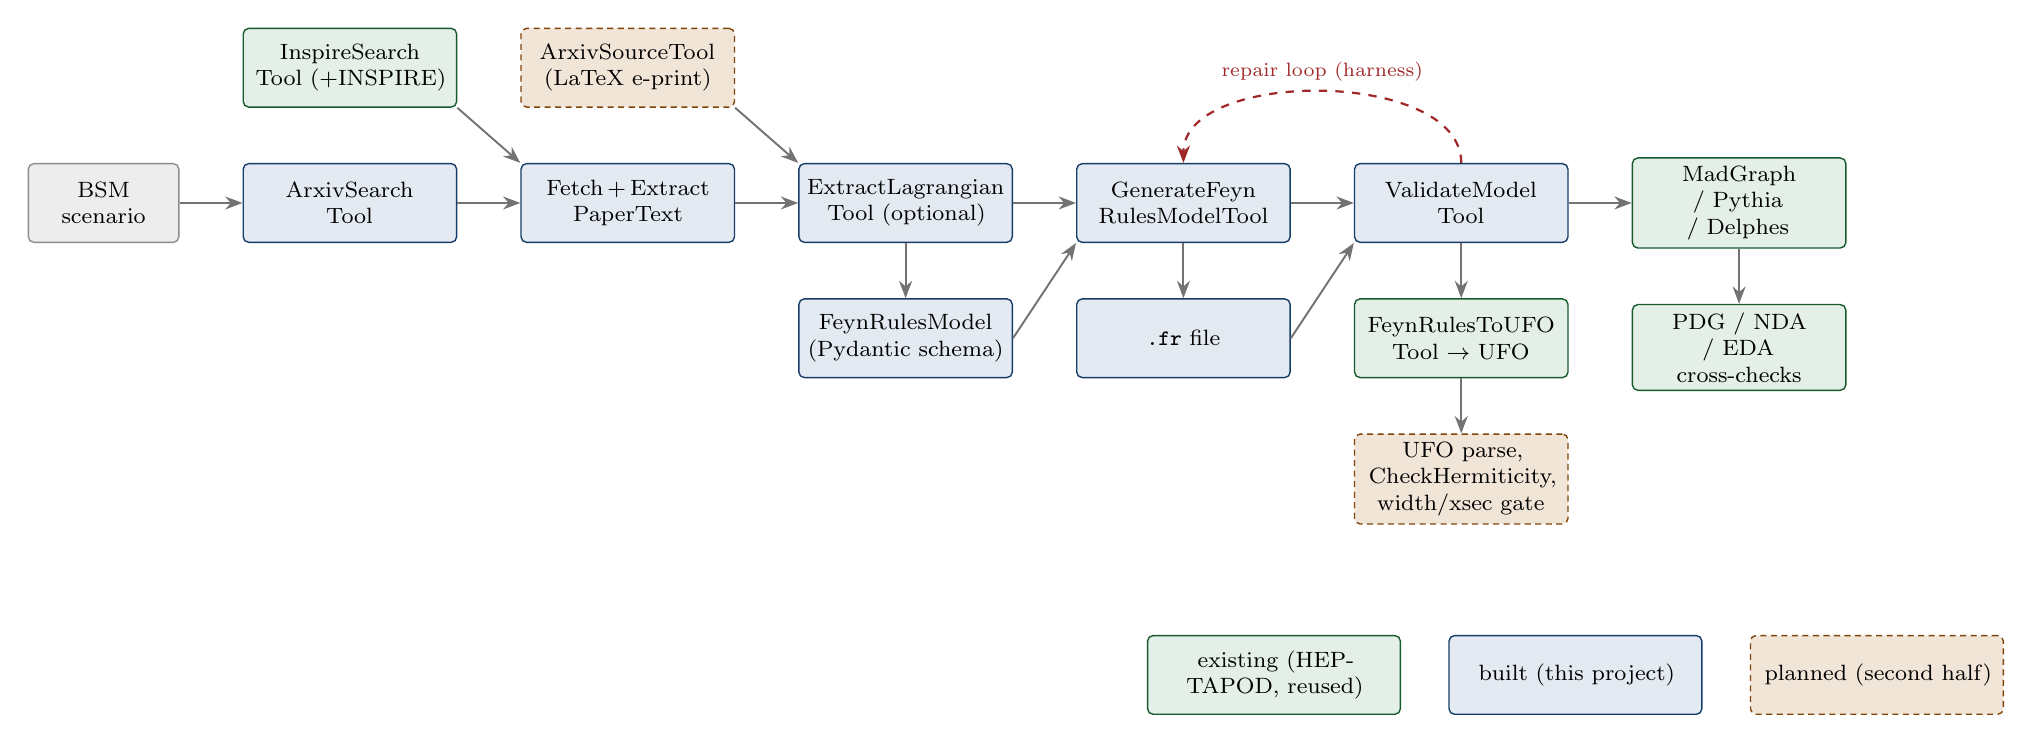
\begin{tikzpicture}[font=\footnotesize, node distance=7mm and 8mm]
  \node[io] (scn) {BSM\\scenario};
  \node[built, right=of scn] (arx) {ArxivSearch\\Tool};
  \node[built, right=of arx] (ing) {Fetch\,+\,Extract\\PaperText};
  \node[built, right=of ing] (ext) {ExtractLagrangian\\Tool (optional)};
  \node[built, right=of ext] (gen) {GenerateFeyn\\RulesModelTool};
  \node[built, right=of gen] (val) {ValidateModel\\Tool};
  \node[existing, right=of val] (down) {MadGraph / Pythia\\/ Delphes};
  \node[existing, above=of arx] (insp) {InspireSearch\\Tool (+INSPIRE)};
  \node[planned, above=of ing] (src) {ArxivSourceTool\\(LaTeX e-print)};
  \node[built, below=of ext] (schema) {FeynRulesModel\\(Pydantic schema)};
  \node[built, below=of gen] (fr) {\code{.fr} file};
  \node[existing, below=of val] (ufo) {FeynRulesToUFO\\Tool $\to$ UFO};
  \node[existing, below=of down] (pdg) {PDG / NDA / EDA\\cross-checks};
  \node[planned, below=of ufo] (deep) {UFO parse,\\CheckHermiticity,\\width/xsec gate};
  \draw[ar] (scn)--(arx); \draw[ar] (arx)--(ing); \draw[ar] (ing)--(ext);
  \draw[ar] (ext)--(gen); \draw[ar] (gen)--(val); \draw[ar] (val)--(down);
  \draw[ar] (insp.south east) -- (ing.north west);
  \draw[ar] (src.south east) -- (ext.north west);
  \draw[ar] (ext) -- (schema);
  \draw[ar] (schema.east) -- (gen.south west);
  \draw[ar] (gen) -- (fr);
  \draw[ar] (fr.east) -- (val.south west);
  \draw[ar] (val) -- (ufo);
  \draw[ar] (ufo) -- (deep);
  \draw[ar] (down) -- (pdg);
  \draw[ar, dashed, draw=gap, line width=0.8pt]
     (val.north) .. controls +(0,12mm) and +(0,12mm) .. (gen.north)
     node[midway, above, font=\scriptsize, text=gap] {repair loop (harness)};
  \node[existing, below left=14mm and -6mm of deep, text width=30mm] (lg1) {existing (HEPTAPOD, reused)};
  \node[built, right=6mm of lg1, text width=30mm] (lg2) {built (this project)};
  \node[planned, right=6mm of lg2, text width=30mm] (lg3) {planned (second half)};
\end{tikzpicture}
\caption{End-to-end workflow. \textcolor{okgreen!70!black}{\textbf{Green}} =
existing HEPTAPOD tools we reuse; \textcolor{accent}{\textbf{blue}} = built and
tested this term; \textcolor{warn}{\textbf{orange, dashed}} = planned. The dashed
red \emph{repair loop} is executed by the driving harness (Figure~1), not by
custom code.}
\end{figure}
\end{landscape}

\subsection{Components: what exists vs.\ what we build on top}

\renewcommand{\arraystretch}{1.15}
\begin{longtable}{@{}p{2.0cm} p{4.4cm} p{1.5cm} p{6.4cm}@{}}
\toprule
\textbf{Stage} & \textbf{Component} & \textbf{Status} & \textbf{Role / key technology} \\
\midrule
\endhead
Harness & Claude Code / Codex / Orchestral & \EX & Swappable driver; owns orchestration $+$ repair loop. \\
Discovery & \code{InspireSearchTool} ($+$10 INSPIRE tools) & \EX & Citation-ranked metadata search; reused unchanged. \\
Discovery & \code{ArxivSearchTool} & \BU & arXiv Atom search (ids, PDF links, abstracts). \\
Ingestion & \code{FetchPaperPDFTool}, \code{ExtractPaperTextTool} & \BU & Sandboxed PDF download (SSRF-guarded) $+$ PyMuPDF full-text. \\
Ingestion & \code{ArxivSourceTool} (LaTeX) & \PL & Primary extraction input from arXiv \code{.tex} e-prints (PDF math is lossy). \\
Extraction & \code{ExtractLagrangianTool} & \BU\,(opt.) & Schema-constrained decode \arw{} \code{FeynRulesModel}; optional---a harness can extract directly. \\
Schema & \code{FeynRulesModel} (Pydantic) & \BU & Central artifact: particles, quantum numbers, parameters, indices; numbers-as-strings preserve rationals ($-1/3$); Lagrangian terms verbatim. \\
Generation & \code{GenerateFeynRulesModelTool} & \BU & Deterministic Jinja2 \arw{} syntactically valid \code{.fr}; round-trips \code{S1\_LQ\_RR.fr}. \\
Validation & \code{ValidateModelTool} & \BU & Drives compile $+$ structural checks; returns structured errors for the repair loop. \\
Validation & \code{FeynRulesToUFOTool} & \EX & Mathematica/FeynRules \code{.fr}\arw{}UFO---the deterministic verifier; reused. \\
Validation & real UFO parse $+$ \code{CheckHermiticity} / spectrum & \PL & Gauge-invariance / symmetry checks surfaced as named pass/fail. \\
Validation & analytic width / cross-section gate & \PL & Reproduce known $\Gamma$, LO $\sigma$ vs.\ published values (tolerance). \\
Downstream & MadGraph / Pythia / Sherpa / Delphes & \EX & Event generation and detector simulation; reused. \\
Cross-checks & PDG, NDA, EDA (Diagrammatica) & \EX & Masses/widths, dimensional-analysis sanity checks; reused. \\
Provenance & Audit trail (prompt) \arw{} \code{audit.json} tool & \BU/\PL & Records sources, extracted terms, conventions, decisions. \\
Benchmark & \code{eval} (scoring $+$ runner) & \BU/\PL & Extraction recall / charge accuracy now; diff-vs-reference-\code{.fr} planned. \\
\bottomrule
\end{longtable}

\subsection{Data flow and design decisions}

The \code{FeynRulesModel} schema is the pipeline's spine: extraction \emph{writes}
it, generation \emph{reads} it, validation \emph{checks} the compiled result
against it.
\begin{itemize}
  \item \textbf{Structure the error-prone blocks; carry the rest verbatim.} The
  schema captures particles, quantum numbers, parameters, and index/gauge
  declarations, numbers stored as strings so $-1/3$ survives exactly; Lagrangian
  terms are verbatim Mathematica, with escape hatches for irregular constructs.
  \item \textbf{Deterministic generation.} Jinja2 renders the \code{.fr}; the LLM
  never hand-writes Mathematica syntax---removing a class of errors that a
  ``let the harness write the \code{.fr}'' design would reintroduce.
  \item \textbf{Schema-constrained extraction.} Output is well-formed or a
  repairable validation error is returned.
  \item \textbf{A real verifier and a harness-run repair loop} (Figure~1).
  \item \textbf{Harness- and model-agnostic, auditable}---the same MCP tools run
  under Claude Code, Codex, or a local Ollama model, with a provenance trail.
\end{itemize}

\section{Novelty and positioning}
\label{sec:novelty}

The \emph{back half} is not novel: ColliderAgent (arXiv:2603.14553) already
automates LaTeX-Lagrangian \arw{} FeynRules \arw{} UFO \arw{} MadGraph, and
MadAgents (arXiv:2601.21015, v3) runs simulation campaigns from a
\emph{user-supplied} PDF. Our contribution is the \textbf{front half}:
model-name-driven literature \emph{discovery} (INSPIRE/arXiv) and extraction of
the Lagrangian \emph{and its conventions} from retrieved paper text with per-term
provenance---which neither does. A second differentiator is architectural:
ColliderAgent ships as Claude-Code-specific \emph{skills}, whereas our capability
is a set of HEPTAPOD \emph{MCP tools} usable from any harness \emph{and} from a
reproducible headless loop---the harness-agnostic design of
Section~\ref{sec:harness}. Related 2026 work, differentiated: \code{bsm\_agent}
(arXiv:2606.21316) constructs Lagrangians from user-specified quantum numbers
(de-novo, not from literature); FERMIACC / ``Albert'' generate theories from
\emph{data} (SARAH, not FeynRules); Denario (arXiv:2510.26887, linked by the
mentors) is a general research-paper agent whose modular design informs our
audit-trail and search agents. The field is moving fast (three overlapping
agentic-HEP systems in H1 2026), so extraction-with-provenance plus a
harness-agnostic tool layer is the durable differentiator.

\section{Design revisions from an adversarial self-review}
\label{sec:doability}

\begin{itemize}
  \item \textbf{Ingest arXiv LaTeX source, not PDF text.} PDF math extraction is
  measurably weak (Nougat/olmOCR rank formulas the worst modality; plain PyMuPDF
  is worse). A \code{.tex} e-print ingestion tool ($\sim$1 week) becomes the
  primary input, PDF as fallback---also a differentiator (MadAgents still uses
  PDFs).
  \item \textbf{Re-scope 2HDM as ``assisted''.} The reference 2HDM is the general
  Higgs-basis model (matrix Yukawas, basis freedom, restriction files). Target
  the restricted CP-conserving type-II 2HDM ($\tan\beta$, $\sin(\beta-\alpha)$) as
  assisted, and keep \textbf{scalar leptoquark} and \textbf{scalar-singlet dark
  matter} as the two fully-automatic targets (satisfying ``$\ge$2 models'').
  \item \textbf{Analytic decay-width reproduction is the primary physics gate.}
  Closed forms exist and are license-cheap: $\Gamma(S_1\!\to\! q\,\ell) =
  |y|^2 m_{\mathrm{LQ}}/16\pi$ (arXiv:1801.07641) and $\Gamma(h\!\to\! SS)$
  (arXiv:1306.4710, whose factor-of-two erratum is a designed test). Cross
  sections are a secondary LO-vs-LO gate with pinned PDF/scale/seed.
  \item \textbf{Plan around the Mathematica/FeynRules license.} FeynRules
  compilation and its gauge checks require a license and cannot run in public CI.
  Split validation: structural checks and comparisons against \emph{published}
  UFO models run license-free in CI, while FeynRules compilation runs on
  mentor/Fermilab infrastructure.
  \item \textbf{Deepen validation.} Replace the name-substring UFO check with real
  \code{particles.py} parsing (name/PDG/charge/spin/color) and add FeynRules
  \code{CheckHermiticity} / \code{CheckDiagonalKineticTerms} /
  \code{CheckMassSpectrum} as named checks.
\end{itemize}

\section{Remaining plan (second half)}
\label{sec:remaining}

\begin{itemize}
  \item Ship the convention catalog (parse the FeynRules DB \code{.fr} files).
  \item Add the arXiv LaTeX-source extraction tool; run the pipeline end-to-end
  on the scalar leptoquark under Claude Code / Codex and commit the artifacts
  (audit, model JSON, \code{.fr}, UFO log).
  \item Deepen \code{ValidateModelTool} (real UFO parsing $+$ FeynRules symmetry
  checks) and add an analytic-width comparison tool.
  \item Rebuild the benchmark to diff against reference DB implementations
  (SLQrules, DMsimp, restricted 2HDM); report per-term extraction
  precision/recall as a headline metric---no prior work measures this task.
  \item Rebase onto upstream HEPTAPOD v2.2.0 (new \code{toolkit.yaml} schema) and
  open a pull request; documentation and worked examples.
\end{itemize}

\section{Evaluation}

\begin{itemize}
  \item \textbf{Extraction accuracy:} per-term precision/recall and
  quantum-number (charge) accuracy vs.\ reference FeynRules implementations.
  \item \textbf{End-to-end validation pass rate:} fraction of benchmark models
  whose \code{.fr} compiles to a UFO \emph{and} reproduces a known width/cross
  section within tolerance.
  \item \textbf{Reproducibility:} pinned-model reruns give a stable tool trace
  and \code{.fr}; a local open model reproduces the workflow (no vendor lock-in).
\end{itemize}

\section{Risks}

Extraction accuracy on real hep-ph prose (sign/normalization/chirality
conventions) is unmeasured---so measuring it is itself a contribution, with slack
budgeted. Sign/normalization errors can pass structural checks and only surface
at the width gate, so repair-loop convergence is the key unknown. The Mathematica
license gates the physics-validation loop (mitigated by the CI split).
Competitive convergence is real; the discovery+provenance and harness-agnostic
angles are the hedge.

\section{Reproducibility}

Code lives on a HEPTAPOD fork (branch \code{feature/lagrangian-extraction}),
registered in \code{toolkit.yaml}/\code{test\_runner.py}; five offline test
suites pass (live LLM/FeynRules paths gated). Setup and a live-demo runbook are
in \code{LAGRANGIAN\_EXTRACTION\_SETUP.md} and \code{DEMO.md}. The MCP tool layer
is driven from Claude Code / Codex (\code{claude mcp add} / \code{codex mcp add})
or the Orchestral web UI---the same tools, a swappable harness.

\end{document}
